\section{VQA Dataset Analysis}
\label{sec:analysis}
%\vspace{\sectionReduceBot}
%%%%%%%%%%%%%%%%%%%%%%%%%%%%%%%%%%%%%%%%%%%%%%%%%%%%%%%%%%%
%%%%%%%%%%%%%%%%%%%%%%%%%%%%%%%%%%%%%%%%%%%%%%%%%%%%%%%%%%%
\begin{figure*}[t]
\centering
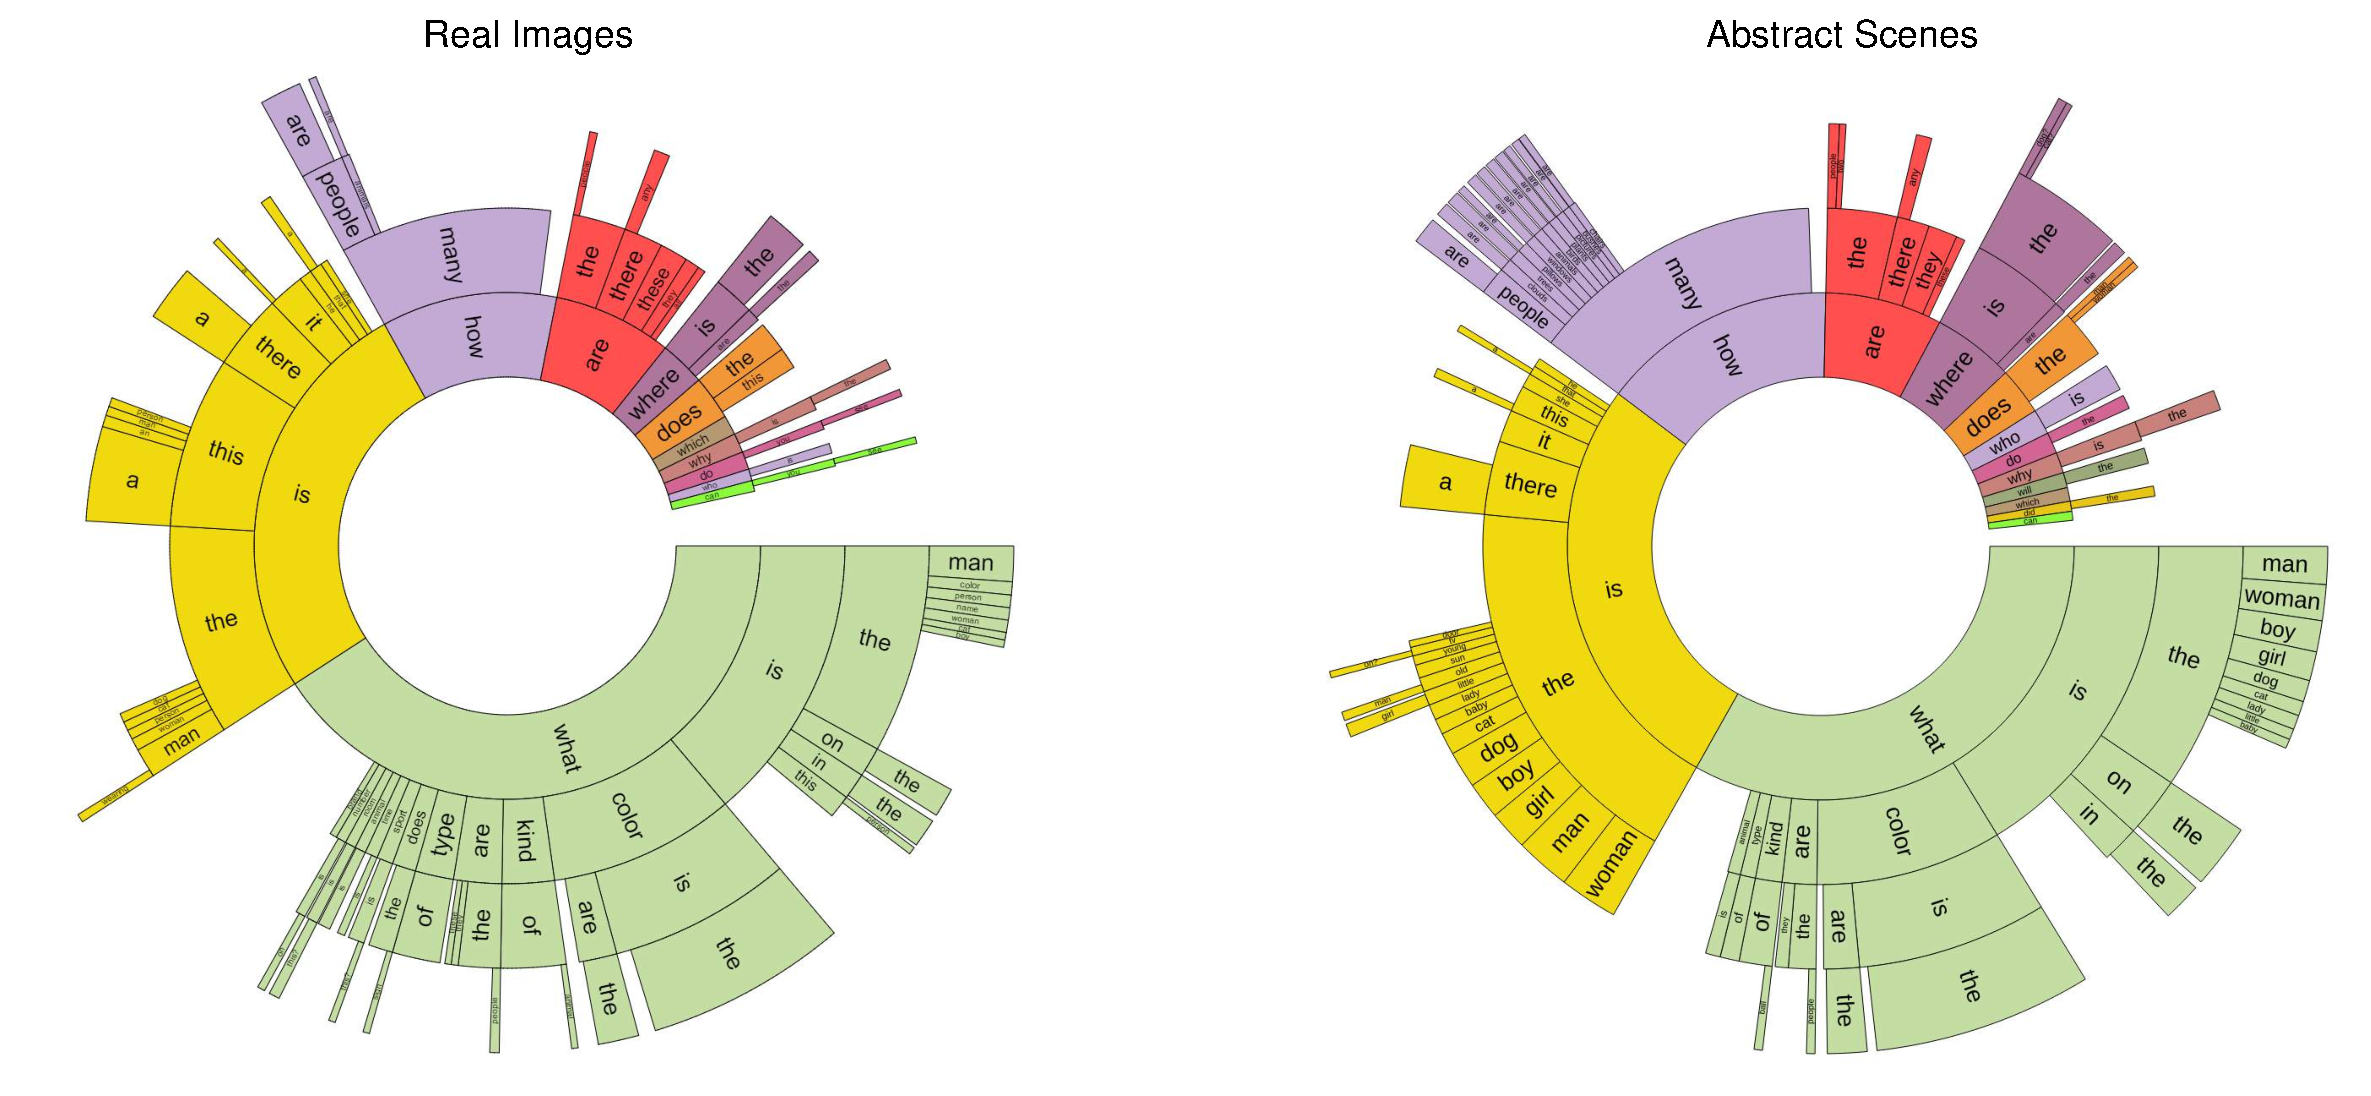
\includegraphics[width=1\linewidth]{figures/QuestionTypes3.pdf}
\caption{Distribution of questions by their first four words for a random sample of 60K questions for real images (left) and all questions for abstract scenes (right). The ordering of the words starts towards the center and radiates outwards. The arc length is proportional to the number of questions containing the word. White areas are words with contributions too small to show. }
%\vspace{-5pt}
\label{fig:QuesCluster}
%\setlength{\belowcaptionskip}{-10pt}
\end{figure*}
%%%%%%%%%%%%%%%%%%%%%%%%%%%%%%%%%%%%%%%%%%%%%%%%%%%%%%%%%%%

In this section, we provide an analysis of the questions and answers in the VQA train dataset.
To gain an understanding of the types of questions asked and answers provided, we visualize
the distribution of question types and answers. We also explore how often the questions may
be answered without the image using just commonsense information. Finally, we analyze whether
the information contained in an image caption is sufficient to answer the questions.

The dataset includes 614,163 questions 
%and a total of 
and 7,984,119 answers (including answers provided by workers with and without 
looking at the image) 
%and without looking at the image) 
for 204,721 images from the MS COCO dataset~\cite{coco} and 150,000 questions with 1,950,000 answers for $50,000$ abstract scenes.

%\textcolor{red}{
%We emphasize that the creation of a dataset of this scale and richness
%is a time consuming process, taking months to complete.
%While the entirety of the dataset has been collected,} at the time of original submission,
%120,520 questions with 270,210 answers for 50,000 MS COCO
%images and 30,000 questions with 79,740 answers for 10,000 abstract scenes had been collected.
%Please refer to the appendix for further details.
%\textcolor{red}{The results in this section still reflect that subset of the final dataset.}
%We emphasize that the creation of a dataset of this scale and richness
%is a time consuming process, taking months to complete.
%By our current estimates,
%approximately 5,000 questions and 40,000 answers are collected per day
%using Amazon Mechanical Turk (AMT).
%The entire dataset will take approximately three months to complete. At the time of submission,
%120,520 questions with 270,210 answers for 50,000 MS COCO
%images and 30,000 questions with 79,740 answers for 10,000 abstract scenes had been collected.
%Please refer to the appendix for further details.


%%%%%%%%%%%%%%%%%%%%%%%%%%%%%%%%%%%%%%%%%%%%%%%%%%%%%%%%%%%
%\vspace{\subsectionReduceTop}
\subsection{Questions}
%\vspace{\subsectionReduceBot}
%%%%%%%%%%%%%%%%%%%%%%%%%%%%%%%%%%%%%%%%%%%%%%%%%%%%%%%%%%%

\textbf{Types of Question.}
Given the structure of questions generated in the English language,
we can cluster questions into different types based on the words that start the question.
\figref{fig:QuesCluster} shows the distribution of questions based on the first four
words of the questions for both the real images (left) and abstract scenes (right).
Interestingly, the distribution of questions is quite similar for both real images and abstract scenes.
This helps demonstrate that the type of questions elicited by the abstract scenes is similar to
those elicited by the real images. There exists a surprising variety of question types,
including ``What is$\ldots$'', ``Is there$\ldots$'', ``How many$\ldots$'', and ``Does the$\ldots$''.
Quantitatively, the percentage of questions for different types is shown in \tableref{tab:typeacc}. Several example questions and answers are shown in \figref{fig:qualResults}.
%\textbf{Sub-Types.}
A particularly interesting type of question is the ``What is$\ldots$'' questions, since they have a
diverse set of possible answers. See the appendix for visualizations for ``What is$\ldots$'' questions.

\textbf{Lengths.}
\figref{fig:QuesLen} shows the distribution of question lengths.
We see that most questions range from four to ten words.


\begin{comment}\begin{table}[h]
{\small
\begin{tabular}{@{\extracolsep{\fill}}p{2cm}|ccccc@{\extracolsep{\fill}}}
%\toprule
Dataset  & Yes & No\\
%\midrule
Real   & 18.21 & 14.06 \\
Abstract & 26.54 & 16.70 \\
\end{tabular}
}
\vspace{5pt}
\caption{Percentage of ``yes'' and ``no'' questions in the real and abstract datasets.}
\label{table:yesno}
%\vspace{\captionReduceBot}
\end{table}
\end{comment}

%%%%%%%%%%%%%%%%%%%%%%%%%%%%%%%%%%%%%%%%%%%%%%%%%%%%%%%%%%%
\begin{figure}[t]
\centering
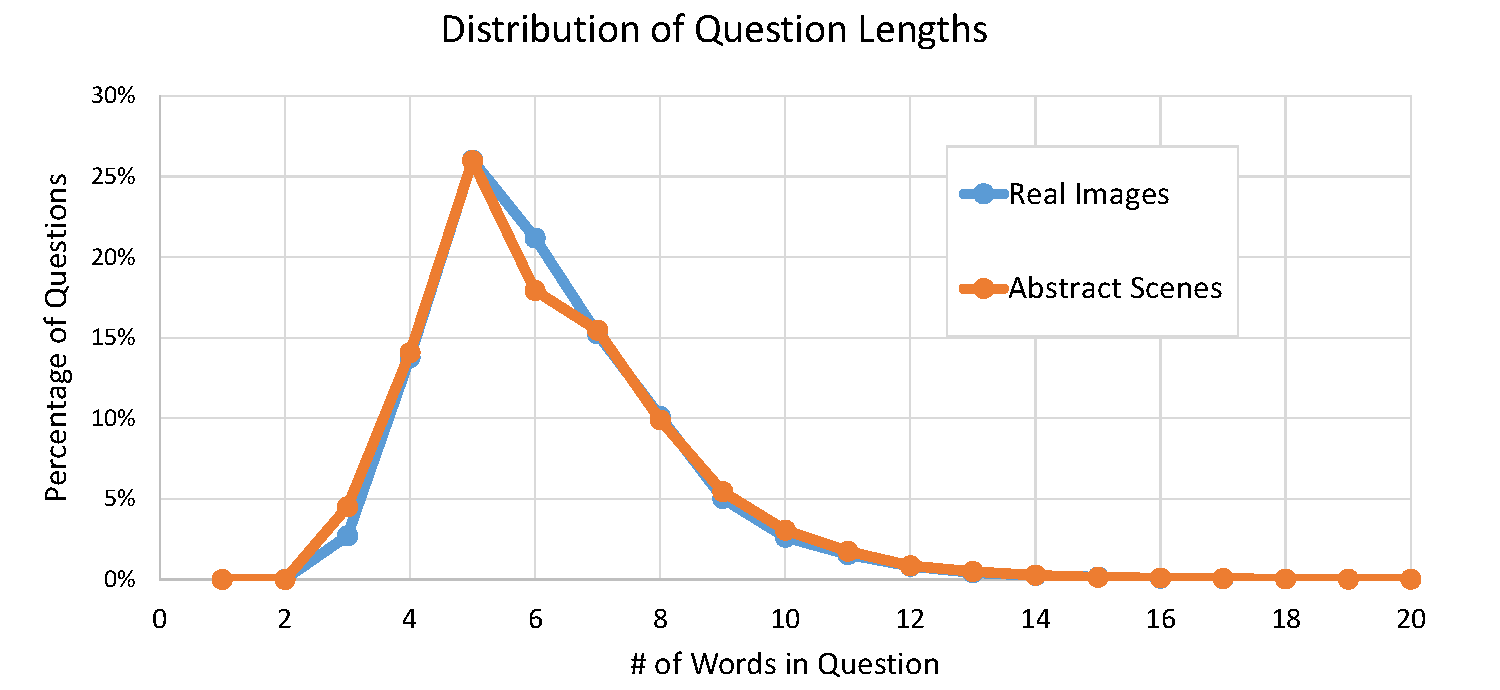
\includegraphics[width=1\linewidth]{figures/Lengths.pdf}
%\vspace{-9pt}
\caption{Percentage of questions with different word lengths for real images and abstract scenes.}
%\vspace{-5pt}
\label{fig:QuesLen}
%\setlength{\belowcaptionskip}{-10pt}
\end{figure}
%%%%%%%%%%%%%%%%%%%%%%%%%%%%%%%%%%%%%%%%%%%%%%%%%%%%%%%%%%%




\begin{figure*}
\centering
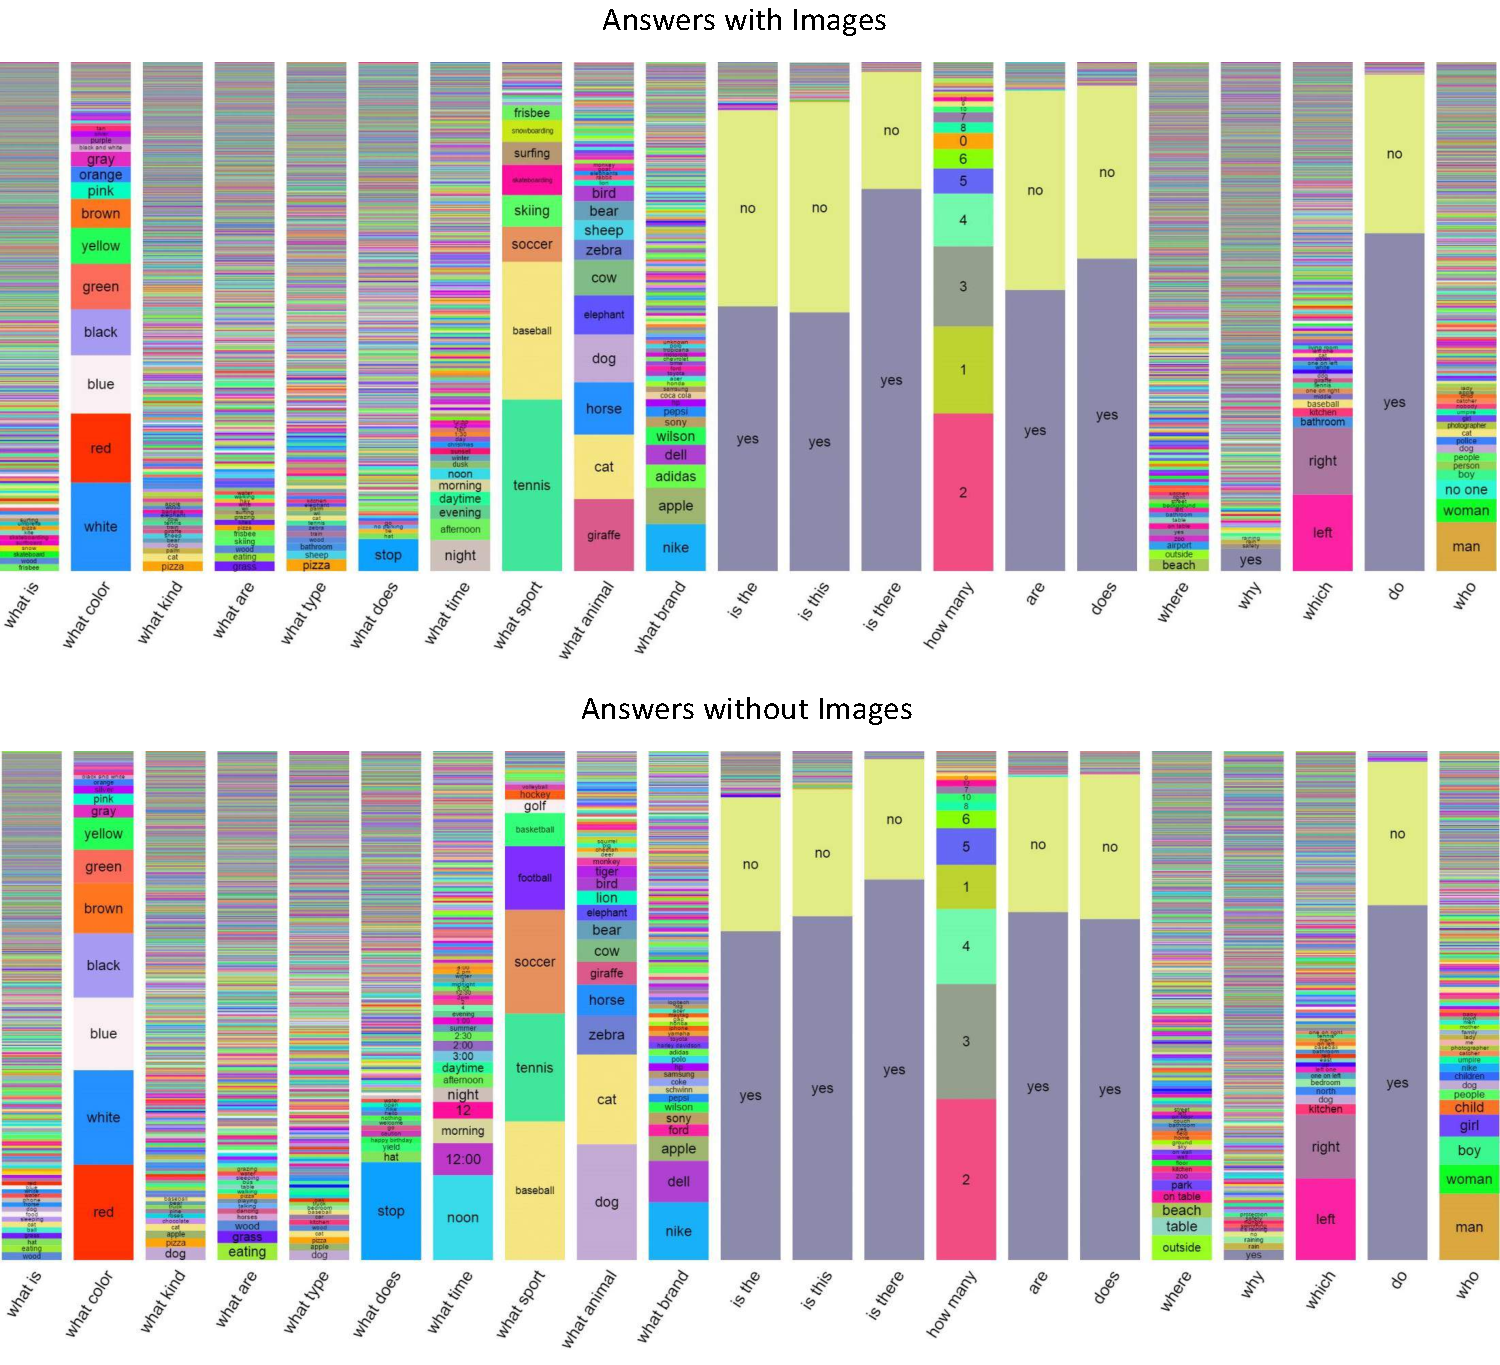
\includegraphics[width=1\linewidth]{figures/answers.pdf}
%\vspace{-5pt}
\caption{Distribution of answers per question type for a random sample of 60K questions for real images when subjects provide answers when given the image (top) and when not given the image (bottom).}
%\vspace{-5pt}
\label{fig:AnsPerQues}
%\setlength{\belowcaptionskip}{-10pt}
\end{figure*}


%%%%%%%%%%%%%%%%%%%%%%%%%%%%%%%%%%%%%%%%%%%%%%%%%%%%%%%%%%%
%\vspace{\subsectionReduceTop}
\subsection{Answers}
%\vspace{\subsectionReduceBot}
%%%%%%%%%%%%%%%%%%%%%%%%%%%%%%%%%%%%%%%%%%%%%%%%%%%%%%%%%%%

%\textbf{Typical Answers for Different Question Types.}
\textbf{Typical Answers.}
%Next, we analyze the answers provided for different question types.
\figref{fig:AnsPerQues} (top) shows the distribution of answers for several question types.
We can see that a number of question types, such as ``Is the\ldots'', ``Are\ldots'', and ``Does\ldots'' are
typically answered using ``yes'' and ``no'' as answers.
%\textcolor{red}{Question types such as ``How many\ldots'' are answered using numbers. $12.31\%$ and $14.48\%$ of the questions are answered using numbers on real images and abstract scenes, respectively.}
Other questions such as ``What is\ldots'' and ``What type\ldots'' have a rich diversity
of responses. Other question types such as ``What color\ldots'' or ``Which\ldots'' have more specialized responses,
such as colors, or ``left'' and ``right''. 
See the appendix for a list of the most popular answers.

\textbf{Lengths.}
Most answers consist of a single word, with the distribution of answers containing one, two, or three words, respectively being $89.32\%$, $6.91\%$, and $2.74\%$ for real images and $90.51\%$, $5.89\%$, and $2.49\%$ for abstract scenes.
%$89.16\%$, $7.00\%$, and $2.77\%$ of answers containing one, two, or three words, respectively.
The brevity of answers is not surprising, since the questions tend to elicit specific
information from the images. This is in contrast with image captions that generically
describe the entire image and hence tend to be longer. The brevity of our answers makes
automatic evaluation feasible. While it may be tempting to believe the brevity of the answers
makes the problem easier, recall that they are human-provided open-ended answers to
open-ended questions. The questions typically require complex reasoning to arrive at these
deceptively simple answers (see \figref{fig:qualResults}).
There are currently 23,234 unique one-word answers in our dataset for real images and 3,770 for abstract scenes.
%There are currently 10,011 unique one-word answers in our dataset.

\textbf{`Yes/No' and `Number' Answers.}
Many questions are answered using either ``yes'' or ``no'' (or sometimes ``maybe'') -- 
$38.37\%$ and $40.66\%$ of the questions on real images and abstract scenes respectively. 
Among these `yes/no' questions, there is a bias towards %answering with 
``yes'' -- %with ``yes'' being preferred %$61.32\%$ and $58.46\%$ 
$58.83\%$ and $55.86\%$ of `yes/no' answers are ``yes'' for real images and abstract scenes. 
Question types such as ``How many\ldots'' are answered using numbers -- 
$12.31\%$ and $14.48\%$ of the questions on real images and abstract scenes are `number' questions. 
``2'' is the most popular answer among the `number' questions, making up 
$26.04\%$ of the `number' answers for real images and $39.85\%$ for abstract scenes. 

\textbf{Subject Confidence.}
When the subjects answered the questions, we asked
``Do you think you were able to answer the question correctly?''.
\figref{fig:ConfScores} shows the distribution of responses. A majority of the answers
were labeled as confident for both real images and abstract scenes. % respectively.

\textbf{Inter-human Agreement.}
Does the self-judgment of confidence correspond to the answer agreement between subjects?
\figref{fig:ConfScores} shows the percentage of questions in which 
(i) $7$ or more, 
(ii) $3-7$, or 
(iii) less than $3$ subjects agree on the answers given their average confidence score 
(0 = not confident, 1 = confident).
As expected, the agreement between subjects increases with confidence.
However, even if all of the subjects are confident the answers may still vary.
This is not surprising since some answers may vary, yet have very similar meaning, such as ``happy'' and ``joyful''.

\begin{figure}[t]
\centering
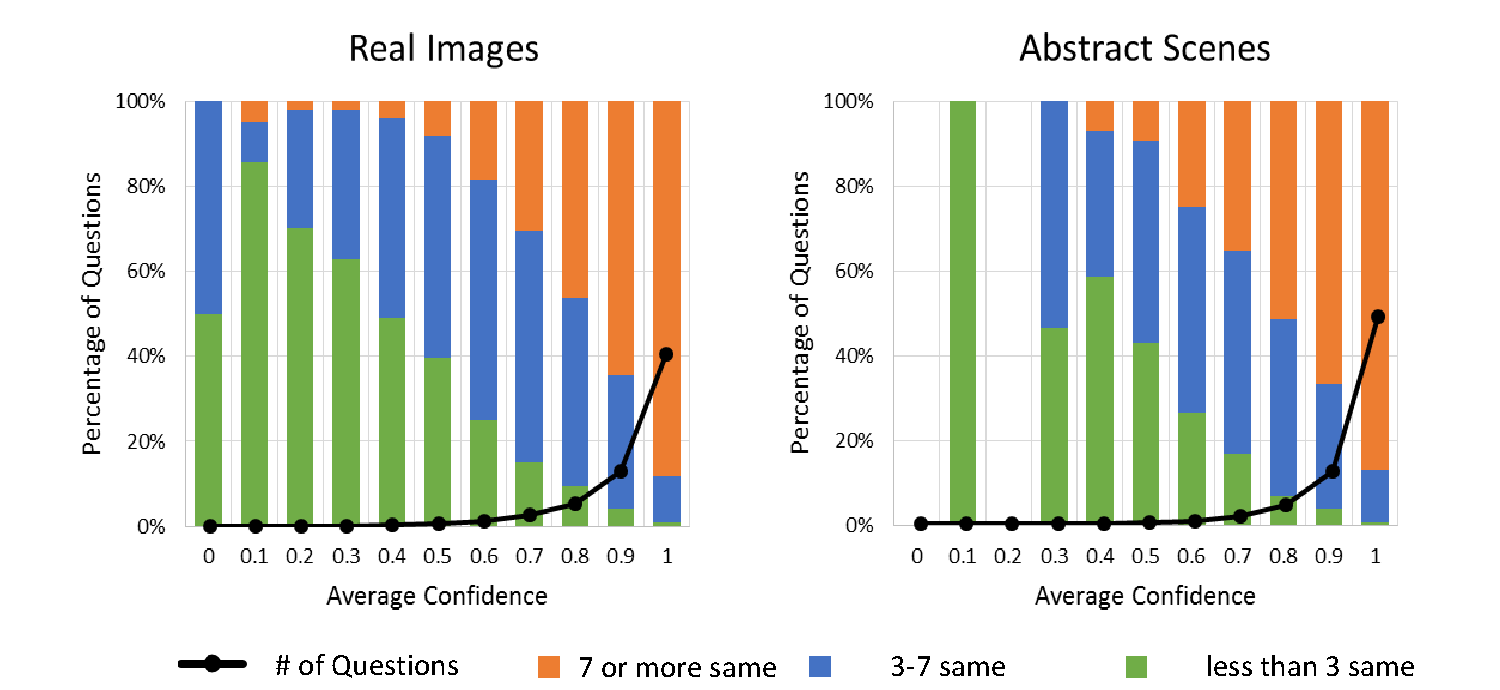
\includegraphics[width=1\linewidth]{figures/Confidence.pdf}
%\vspace{-5pt}
\caption{Number of questions per average confidence score (0 = not confident, 1 = confident) for real images and abstract scenes (black lines). Percentage of questions where 7 or more answers are same, 3-7 are same, less than 3 are same (color bars). }
%\vspace{-7pt}
\label{fig:ConfScores}
%\setlength{\belowcaptionskip}{-10pt}
\end{figure}

As shown in \tableref{table:commonsense_acc} (Question + Image), there is significant inter-human
agreement in the answers for both real images ($83.30\%$) and abstract scenes ($87.49\%$). 
%when humans are provided both the question and image while answering the question.
Note that on average each question has $2.70$ unique answers for real images and $2.39$ for abstract scenes. 
The agreement is significantly higher ($>95\%$) for \quotes{yes/no} questions and lower for other questions ($<76\%$), possibly due to the fact that we perform exact string matching and do not account for synonyms, plurality, \etc. Note that the automatic determination of synonyms is a difficult problem, since the level of answer granularity can vary across questions.




%%%%%%%%%%%%%%%%%%%%%%%%%%%%%%%%%%%%%%%%%%%%%%%%%%%%%%%%%%%
%\vspace{\subsectionReduceTop}
\subsection{Commonsense Knowledge}
\label{sec:cs}
%\vspace{\subsectionReduceBot}
%%%%%%%%%%%%%%%%%%%%%%%%%%%%%%%%%%%%%%%%%%%%%%%%%%%%%%%%%%%
\begin{figure*}[t]
 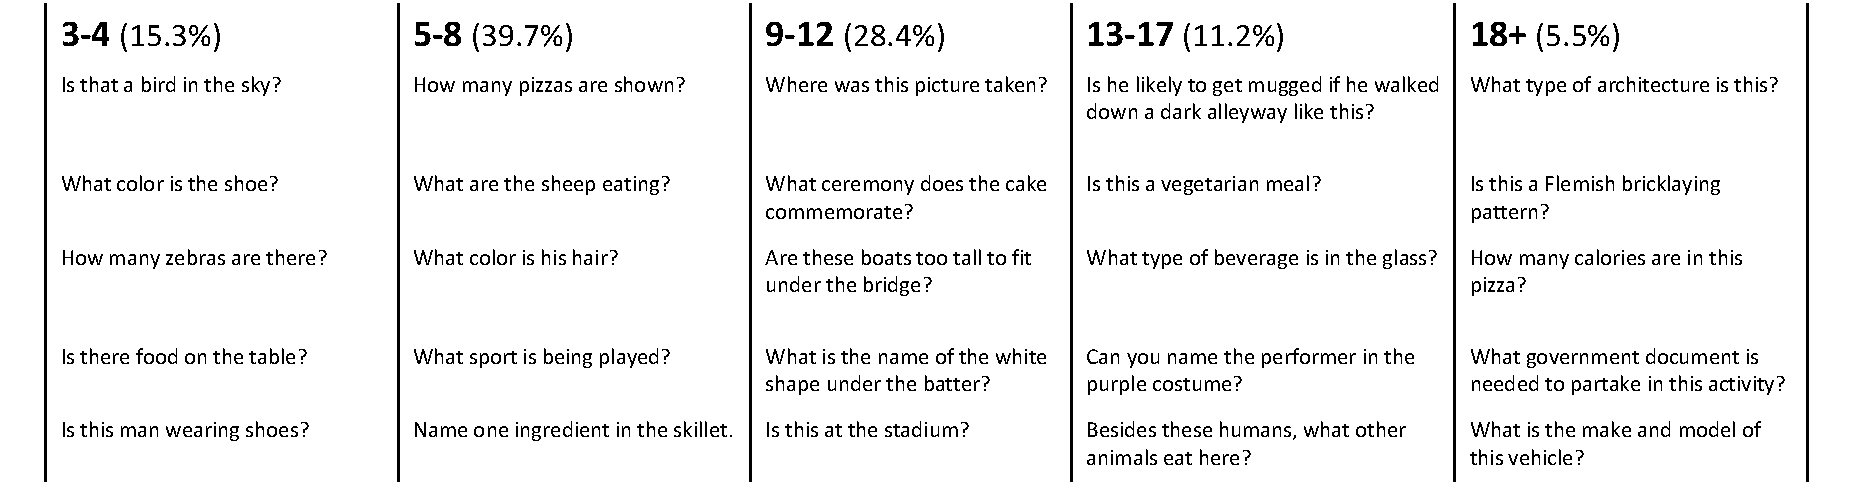
\includegraphics[width=\linewidth]{figures/age.pdf}
 \centering
\caption{\small Example questions judged by Mturk workers to be answerable by different age groups. The percentage of questions falling into each age group is shown in parentheses.}
 \label{fig:age}
 \end{figure*}
 	
\textbf{Is the Image Necessary?}
%Can the questions be answered using commonsense knowledge alone without the need for an image,
%\eg, ``What is the color of the sheep?''?
Clearly, some questions can sometimes be
answered correctly using commonsense knowledge alone without the need for an image,
\eg, ``What is the color of the fire hydrant?''.
We explore this issue by asking three subjects to answer
the questions \emph{without seeing the image} (see the examples in blue in \figref{fig:qualResults}).
In \tableref{table:commonsense_acc} (Question), we show the percentage of questions for which
the correct answer is provided over all questions, ``yes/no'' questions, and the other questions that
are not ``yes/no''. For ``yes/no'' questions, the human subjects respond better than chance.
For other questions, humans are only correct about $21\%$ of the time. This demonstrates that
understanding the visual information is critical to VQA and that commonsense information alone is not sufficient.

To show the qualitative difference in answers provided with and without images,
we show the distribution of answers for various question types in \figref{fig:AnsPerQues} (bottom).
The distribution of colors, numbers, and even ``yes/no'' responses is surprisingly different for answers
with and without images.
 
\textbf{Which Questions Require Common Sense?}
In order to identify questions that require commonsense reasoning to answer, we conducted 
two AMT studies (on a subset 10K questions from the real images of VQA trainval) asking subjects --
\begin{compactenum} 
\item Whether or not they believed a question required commonsense to answer the question, and 
\item The youngest age group that they believe a person must be in order to be able to correctly answer the question -- 
toddler (3-4), 
younger child (5-8), 
older child (9-12), 
teenager (13-17), 
adult (18+).
\end{compactenum}
Each question was shown to 10 subjects. We found that 
for $47.43\%$ of questions 3 or more subjects voted `yes' to commonsense, 
($18.14\%$: 6 or more).  
In the `perceived human age required to answer question' study, we found the following distribution of responses: 
toddler: $15.3\%$,
younger child: $39.7\%$, 
older child: $28.4\%$, 
teenager: $11.2\%$, 
adult: $5.5\%$.
In Figure \ref{fig:age} we show several questions for which a majority of subjects picked the specified age range. Surprisingly the perceived age needed to answer the questions is fairly well distributed across the different age ranges. As expected the questions that were judged answerable by an adult (18+) generally need specialized knowledge, whereas those answerable by a toddler (3-4) are more generic.
 
We measure the degree of commonsense required to answer a question as the percentage of subjects (out of 10) who voted ``yes'' in our ``whether or not a question requires commonsense'' study.
A fine-grained breakdown of average age and average degree of common sense (on a scale of $0-100$) required to answer a question is shown in \tableref{tab:typeacc}. The average age and the average degree of commonsense across all questions is $8.92$ and $31.01\%$ respectively. 

%\arxiv{To compute average age and average degree of commonsense across questions, we first compute the average age and average degree of commonsense (binary response scaled to $0-100$) per question (by taking average across 10 subjects for each question) and then take average across questions.} 

It is important to distinguish between:
\begin{compactenum}
\item How old someone needs to be to be able to answer a question correctly,  and
\item How old people \emph{think} someone needs to be to be able to answer a question correctly. 
\end{compactenum}

Our age annotations capture the latter -- perceptions of MTurk workers in an uncontrolled environment. As such, the relative ordering of question types in \tableref{tab:typeacc} is more important than absolute age numbers.
%The relative ordering of question types is more important than the absolute age numbers. It is important to note that the age annotations we have collected are just perceived ages: how old people -- untrained MTurk workers in an uncontrolled environment -- \emph{think} someone needs to be to be able to answer a question correctly.}
The two rankings of questions in terms of common sense required according to the two studies 
were largely correlated (Pearson's rank correlation: 0.58). 

%%%%%%%%%%%%%%%%%%%%%%%%%%%%%%%%%%%%%%%%%%%%%%%%%%%%%%%%%%%
\begin{table}[t]
\setlength{\tabcolsep}{3.2pt}
{\small
\begin{center}
%\begin{tabular}{@{}llccc@{}}
%\toprule
%Dataset & Input & All & Yes/No & Other \\
%%\hline
%\midrule
%    & Question & 40.81 & 67.60 & 21.22 \\
%Real   & Question + Caption* & 57.47 & 78.97 & 44.41 \\
%    & Question + Image & 83.30 & 95.77 & 72.67 \\
%%\hline
%\midrule
% & Question & 43.27 & 66.65 &  23.66 \\
%Abstract & Question + Caption* & 54.34 & 74.70 & 40.18 \\
% & Question + Image & 87.49 & 95.96 & 75.33 \\
%\bottomrule
%\end{tabular}
\begin{tabular}{@{}llcccc@{}}
\toprule
Dataset & Input & All & Yes/No & Number & Other \\
%\hline
\midrule
    & Question & 40.81 & 67.60 & 25.77 & 21.22 \\
Real   & Question + Caption* & 57.47 & 78.97 & 39.68 & 44.41 \\
    & Question + Image & 83.30 & 95.77 & 83.39 & 72.67 \\
%\hline
\midrule
 & Question & 43.27 & 66.65 & 28.52 & 23.66 \\
Abstract & Question + Caption* & 54.34 & 74.70 & 41.19 & 40.18 \\
 & Question + Image & 87.49 & 95.96 & 95.04 & 75.33 \\
\bottomrule
\end{tabular}
\end{center}
}
%\vspace{-7pt}
\caption {Test-standard accuracy of human subjects when asked to answer the 
question without seeing the image (Question), 
seeing just a caption of the image and not the image itself (Question + Caption), 
and seeing the image (Question + Image). 
Results are shown for all questions, ``yes/no'' \& ``number'' questions, and other questions 
that are neither answered ``yes/no'' nor number. 
All answers are free-form and not multiple-choice. 
*\hspace{1pt}These accuracies are evaluated on a subset of 3K train questions (1K images).}
% \textcolor{red}{and are not directly comparable to the corresponding numbers in older version.}}
\label{table:commonsense_acc}
%\vspace{\captionReduceBot}
%\vspace{-5pt}
\end{table}
%%%%%%%%%%%%%%%%%%%%%%%%%%%%%%%%%%%%%%%%%%%%%%%%%%%%%%%%%%%


%%%%%%%%%%%%%%%%%%%%%%%%%%%%%%%%%%%%%%%%%%%%%%%%%%%%%%%%%%%
%\vspace{\subsectionReduceTop}
\subsection{Captions \textbf{\vs} Questions}
%\vspace{\subsectionReduceBot}
%%%%%%%%%%%%%%%%%%%%%%%%%%%%%%%%%%%%%%%%%%%%%%%%%%%%%%%%%%%


Do generic image captions provide enough information to answer the questions?
\tableref{table:commonsense_acc} (Question + Caption) shows the percentage of questions answered
correctly when human subjects are given the question and a human-provided caption
describing the image, but not the image. As expected, the results are better than when humans are shown the questions alone.
However, the accuracies are significantly lower than when subjects are shown the actual image.
This demonstrates that in order to answer the questions correctly, deeper image understanding 
(beyond what image captions typically capture) is necessary. In fact, we find that the distributions of nouns, verbs, and adjectives mentioned in captions is statistically significantly different from those mentioned in our questions + answers (Kolmogorov-Smirnov test, $p<.001$) for both real images and abstract scenes. See the appendix for details. 
%This motivates the VQA task as a way to learn further information about visual scenes.